\section{Durchführung}
\label{sec:Durchführung}


\subsection{Aufbau}
Der Versuchsaufbau besteht aus einer Grundplatte mit vier rechteckigen Stäben, die an einer Seite von einem Peltier-Element simultan geheizt oder gekühlt werden.
Die Stäbe sind aus drei verschiedenen Materialien:  Aluminium, Edelstahl und zweimal Messing, mit verschiedenen Breiten.
Zusätzlich sind an jedem Stab zwei Thermoelemente, welche die Temperatur an verschiedenen Stellen der Stäbe messen, zu sehen in\autoref{fig:Versuchsaufbau}.
Die Thermoelemente sind verbunden mit einem GLX Datenlogger (\autoref{fig:GLX}), welcher die Temperaturen aufnimmt und in eine Tabelle überführt.
Zuletzt gibt es auch eine Spannungsquelle, welche bei der statischen Methode eine Betriebspannung von $5\si{V}$ auf das Heizelement überträgt. 
Bei der der dynamischen Methode wird sie auf $8\si{V}$ eingestellt. Bei beidem wird ein maximaler Strom angelegt .
Wie man in \autoref{fig:Versuchsaufbau} sieht sind die Thermoelement durchnummeriert, wobei gilt:
\begin{align}
    T1 &= \text{Messing dick fern} \notag \\
    T2 &= \text{Messing dick nah} \notag \\
    T3 &= \text{Messing dünn nah} \notag \\
    T4 &= \text{Messing dünn fern} \notag \\
    T5 &= \text{Aluminium fern} \notag \\
    T6 &= \text{Aluminium nah} \notag \\
    T7 &= \text{Edelstahl nah} \notag \\
    T8 &= \text{Edelstahl fern} \notag
\end{align}
\begin{figure}[H]
    \centering
    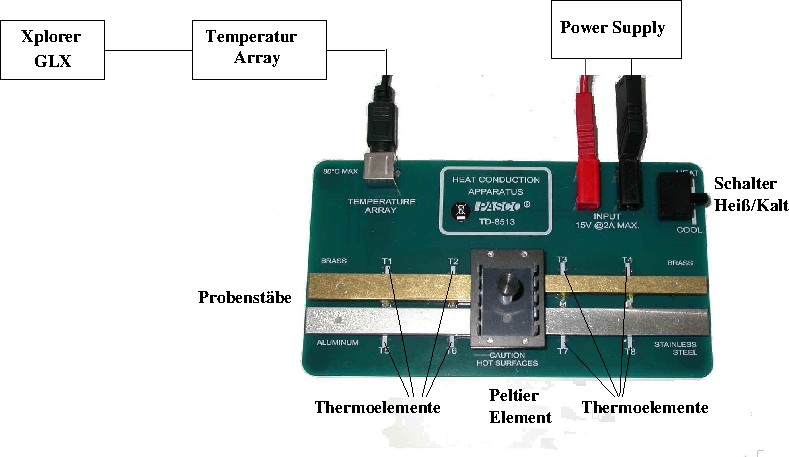
\includegraphics{content/Abb_1.pdf}
    \caption{Grundplatte mit Aluminium, Edelstahl und zweimal Messing\cite[3]{V204}}
    \label{fig:Versuchsaufbau}
\end{figure}

\subsection{Statische Methode}
\label{subsec:durch_stat}
An allen acht Thermoelementen wird der Temperaturverlauf in Abhängigkeit der Zeit gemessen.
Dafür wird die Abtastrate beim GLX auf $\Delta t_{GLX} = 5\si{s}$ Sekunden gestellt.
Es wird solange gemessen bis das Thermoelement $T7$ $\qty{45}{\degreeCelsius}$ anzeigt.
Während des Heizvorgangs werden Isolierungen über die Stäbe gelegt, damit der Wärmeaustausch mit der Umgebung verringert wird.
Nach der Messung werden die Stäbe gekühlt, bis deren Temperaturen maximal $\qty{30}{\degreeCelsius}$ betragen.

\subsection{Dynamische Methode}
\label{subsec:durch_dyn}
Ein anderer Name für die folgende Methode ist das Angström-Messverfahren.
Dabei werden die Probenstäbe periodisch geheizt.
Die Abtastrate wird auf $\Delta t_{GLX} = 2\si{s}$ geändert.\\
Während der ersten Messung beträgt die Periodendauer $80\si{s}$, wobei jeweils $40\si{s}$ geheizt und $40\si{s}$ gekühlt wird.
Während gekühlt wird muss das Peltier-Element auf "COOL" gestellt werden und die Wärmeisolatoren werden abgenommen.
Diese Messung geht über $10$ Perioden.\\
Die zweite Messung wird analog durchgeführt. 
Die Periodendauer beträgt nun jedoch $200 \si{s}$ und die Messung endet, wenn eines der Thermoelemente $\qty{80}{\degreeCelsius}$ erreicht.

\begin{figure}[H]
    \centering
    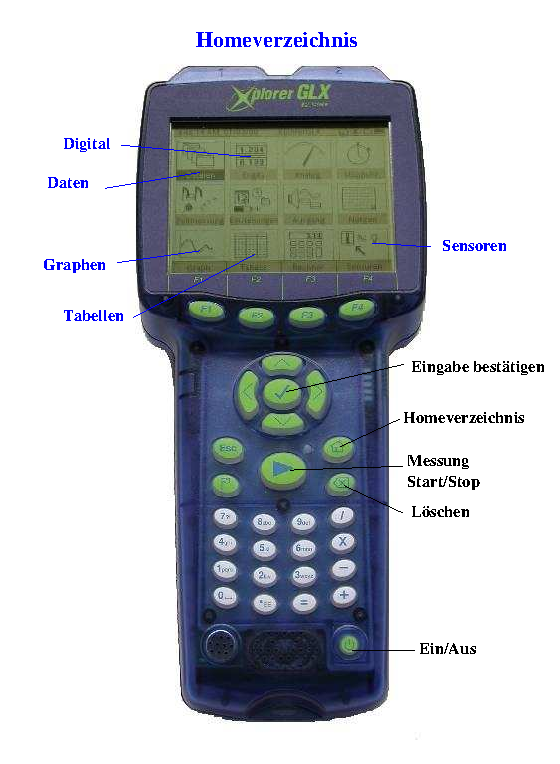
\includegraphics[height=11cm]{content/Abb_2.pdf}
    \caption{Xplore GLX\cite[5]{V204}}
    \label{fig:GLX}
\end{figure}

